\documentclass[12pt]{article}
\usepackage[margin=1in]{geometry}
\usepackage{amsmath}
\usepackage{amssymb}
\usepackage{float}
\usepackage{listings}
\usepackage{mathtools}
\usepackage{graphicx}
\usepackage[hidelinks]{hyperref}
\usepackage[noabbrev,capitalize,nameinlink]{cleveref}
\usepackage{natbib}
\usepackage{setspace}
\usepackage{tikz-cd}

\newcommand{\argmin}{\ensuremath{\mathop{\arg\min}\limits}}
\DeclarePairedDelimiter{\abs}{\lvert}{\rvert}

\title{Automatic Wound Analysis with Siamese Network}
\author{Alex Ruan \\ \texttt{runalex01@gmail.com} \and Siwei Wang \\ \texttt{siweiw9@gmail.com}}
\date{\today}

\begin{document}
\maketitle
\onehalfspacing

\section{Data Preprocessing} \label{sec:data_preprocessing}

Our system expects standard 3-channel images as input (dimensions \(W \times H \times 3\)). We trained our model on images consisting of a rat's abdominal section with one or more wounds. The background was white, and the rat was placed next to a ruler. However, the model can be trained on any labelled dataset to suit a variety of applications.

Each image is resized to a uniform \(40 \times 40 \times 3\) using bicubic interpolation. For best results, we recommend that input images be larger than this size. We then apply a Gaussian blur with a radius of 2. The Siamese model expects resampled and blurred images as input when predicting labels.

During training, the model expects image pairs. The training set is generated by taking all distinct image pairs and labelling the pair with 1 or 0 if the images have the same or different labels, respectively. Suppose our dataset consists of \(N\) labelled images with \(K\) possible labels. We represent the dataset as image-label pairs \((X_i, y_i)\) with \(0 \leq i < N\), \(X_i \in [0, 1]^{40 \times 40 \times 3}\), and \(0 \leq y_i < K\). We generate \(\binom{N}{2}\) pairs of the form \([(X_i, X_j), \delta(y_i, y_j)]\) where \(\delta\) denotes Kronecker delta and \(i \neq j\). Define \(N_i\) as the number of times label \(i\) appears in the training set. Then there are
\begin{equation}
    \sum_{i = 0}^{K - 1} \binom{N_i}{2} \label{eq:same_pairs}
\end{equation}
pairs with label 1. For a reasonably balanced dataset with \(K > 2\), this number will usually be less than half of \(\binom{N}{2}\). The resulting class imbalance is addressed by assigning appropriate class weights during training.

\section{Model Architecture} \label{sec:model_architecture}

\subsection{Overview} \label{subsec:overview}

Label predictions are the result of a 2-step process. The input image is first encoded as a vector representation. The encoding is then compared against a ``typical'' representation for each label. This comparison is carried out with a custom distance metric. The model predicts the label corresponding to the closest representation. In symbols, the model consists of an encoder \(\mathcal{E} \colon [0, 1]^{40 \times 40 \times 3} \to \mathbf{R}^{2048}\), a distance metric \(\mathcal{D} \colon \mathbf{R}^{2048} \times \mathbf{R}^{2048} \to (0, 1)\), and \(K\) ``typical'' representations \(C_0, \dotsc, C_{K - 1}\) with \(C_i \in \mathbf{R}^{2048}\). Given input image \(I \in [0, 1]^{40 \times 40 \times 3}\), the model predicts label
\begin{equation}
    \argmin_{i = 0}^{K - 1} \mathcal{D}(\mathcal{E}(I), C_i) \label{eq:prediction}
\end{equation}
We can interpret the prediction process as a generalization of \(K\)-means. The image \(I\) derives its label by comparing its representation \(\mathcal{E}(I)\) against against \(K\) ``centroids'' and choosing the closest one, where distance is defined by \(\mathcal{D}\).

To train the model, we construct a siamese network with contrastive loss. We would like \(P_{ij} \coloneqq \mathcal{D}(\mathcal{E}(X_i), \mathcal{E}(X_j))\) to approximate \(Y_{ij} \coloneqq \delta(y_i, y_j)\). Note that this problem is a binary classification task with instance \((X_i, X_j)\) and label \(Y_{ij}\). Hence, we use cross-entropy loss \(\mathcal{L}\), which is defined as
\begin{equation}
    \mathcal{L}[(X_i, X_j), Y_{ij}] \coloneqq -Y_{ij} \log P_{ij} - (1 - Y_{ij}) \log (1 - P_{ij}) \label{eq:cross_entropy}
\end{equation}
to tune our model parameters. The forward pass of the training process is summarized in the diagram below.
\begin{equation*}
    \begin{tikzcd}
        X_i \arrow[rr, "\text{encode}"] &  & \mathcal{E}(X_i) \arrow[rrd, "\text{dist}", bend left]   &  &                                  &  & Y_{ij} \arrow[d]                  \\
        &  &                                                          &  & P_{ij} \arrow[rr, "\text{loss}"] &  & {\mathcal{L}[(X_i, X_j), Y_{ij}]} \\
        X_j \arrow[rr, "\text{encode}"] &  & \mathcal{E}(X_j) \arrow[rru, "\text{dist}"', bend right] &  &                                  &  &
    \end{tikzcd} \label{eq:training}
\end{equation*}

We compiled our model with an Adams optimizer (initial learning rate of \(5 \times 10^{-5}\)), a batch size of 5, and saved the model with the lowest validation loss over 30 epochs.

\subsection{The Encoder} \label{subsec:the_encoder}

We use a deep CNN similar to \citet{tds} to encode an image \(I\) as a vector representation. The architecture is fairly standard, consisting of a series of convolutions with ReLU activation followed by max pools. At the end, the image is flattened and passed through a fully connected layer with sigmoid activation. A diagram of the encoder is displayed in \cref{fig:encoder}.

\begin{figure}[H]
    \centering
    \caption{Encoder (CNN) Architecture}
    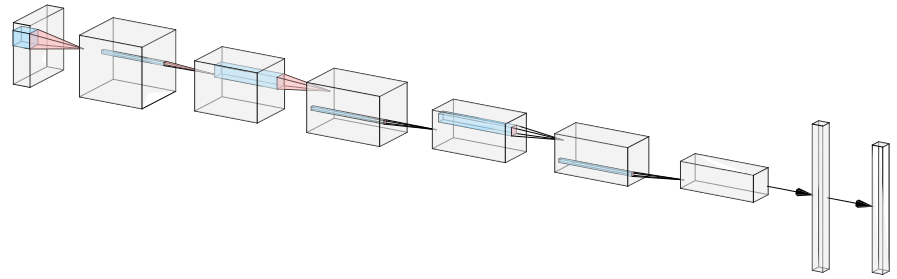
\includegraphics[width=.9\textwidth]{encoder.png}
    \label{fig:encoder}
\end{figure}

The more detailed Keras model summary is reproduced below.
\begin{lstlisting}
_________________________________________________________________
Layer (type)                 Output Shape              Param #
=================================================================
conv2d (Conv2D)              (None, 40, 40, 64)        15616
_________________________________________________________________
max_pooling2d (MaxPooling2D) (None, 20, 20, 64)        0
_________________________________________________________________
conv2d_1 (Conv2D)            (None, 20, 20, 128)       401536
_________________________________________________________________
max_pooling2d_1 (MaxPooling2 (None, 10, 10, 128)       0
_________________________________________________________________
conv2d_2 (Conv2D)            (None, 10, 10, 128)       409728
_________________________________________________________________
max_pooling2d_2 (MaxPooling2 (None, 5, 5, 128)         0
_________________________________________________________________
conv2d_3 (Conv2D)            (None, 5, 5, 256)         295168
_________________________________________________________________
flatten (Flatten)            (None, 6400)              0
_________________________________________________________________
dense (Dense)                (None, 2048)              13109248
=================================================================
\end{lstlisting}

\subsection{The Distance Metric} \label{subsec:the_distance_metric}

Define a component-wise absolute value function \(\alpha \colon \mathbf{R}^n \to \mathbf{R}^n\) given by \((v_1, \dotsc, v_n) \mapsto (\abs{v_1}, \dotsc, \abs{v_n})\). The distance between two representation vectors \(U, V \in \mathbf{R}^{2048}\) is computed by passing \(\alpha(U - V)\) through a fully-connected layer \(F\) with a single output node and sigmoid activation. Then \(\mathcal{D}(U, V) \coloneqq F \circ \alpha(U - V)\). This is the approach used by \citet{cmu}.

The intuition is that we wish to jointly learn an encoding \(\mathcal{E}\) and a ``difference'' interpreter \(F\) that maps images with the same label close together and maps images with different labels far apart. Recall that \(F \coloneqq S \circ T\) consists of an affine transformation \(T \colon \mathbf{R}^{2048} \to \mathbf{R}\) followed by sigmoid activation \(S\). Hence, we see that \(F\) learns to affinely map large differences to very positive values and map small differences to very negative values. Then, \(S\) squeezes these values into the \((0, 1)\) range.

In this case, \(\alpha(U - V)\) quantifies how different the representations \(U\) and \(V\) are from one another. More rigorously, the \(L^1\) norm of \(\alpha(U - V)\) captures the \(L^1\) distance separating \(U\) and \(V\). Hence, we may interpret \(T\) as assigning a weight to each of the 2048 components that comprise a representation vector. This means that we can penalize a difference in certain components more heavily than in others.

The ``typical'' representations \(C_0, \dotsc, C_{K - 1}\) are computed after the model is trained. We used the mean encoding of the training images from each label.
\begin{equation}
    C_i \coloneqq \frac{1}{N_i} \sum_{j = 0}^{N - 1} \delta(y_j, i) \cdot \mathcal{E}(X_j) \label{eq:typical_rep}
\end{equation}
In this sense, \(C_i\) should be close to most images with label \(i\) and far away from most images with label \(j \neq i\), as measured by \(\mathcal{D}\).

\bibliographystyle{abbrvnat}
\bibliography{wound}
\end{document}
